\documentclass[12pt,a4paper]{article}
\usepackage[utf8]{inputenc}
\usepackage[catalan]{babel}
\usepackage{graphicx}
\usepackage{geometry}
\usepackage{fancyhdr}
\usepackage{tabularx}
\usepackage{lastpage}
\usepackage{enumitem}
\usepackage{amsmath}
\usepackage{amssymb}
\usepackage{xcolor}
\usepackage{mdframed}

% ============================================================
%  SOLUCIONS: canvia "true" per "false" per ocultar-les
% ============================================================
\newif\ifsolutions
\solutionstrue   % <--- CANVIA A \solutionsfalse PER OCULTAR
% ============================================================

% Entorn de solució (caixa verda)
\newmdenv[
  linecolor=green!50!black,
  backgroundcolor=green!5,
  frametitle={\textcolor{green!50!black}{\textbf{Solució}}},
  frametitlebackgroundcolor=green!15,
  skipabove=6pt,
  skipbelow=6pt,
  innertopmargin=8pt,
  innerbottommargin=8pt,
]{soluciobox}

% Macro per incloure solucions condicionalment
\newcommand{\solucio}[1]{%
  \ifsolutions
    \begin{soluciobox}
      #1
    \end{soluciobox}
  \fi
}

% 1. MARGES I CAPÇALERA
\geometry{top=4cm, bottom=3cm, left=2cm, right=2cm, headheight=2.5cm}

\pagestyle{fancy}
\fancyhf{}
\fancyhead[L]{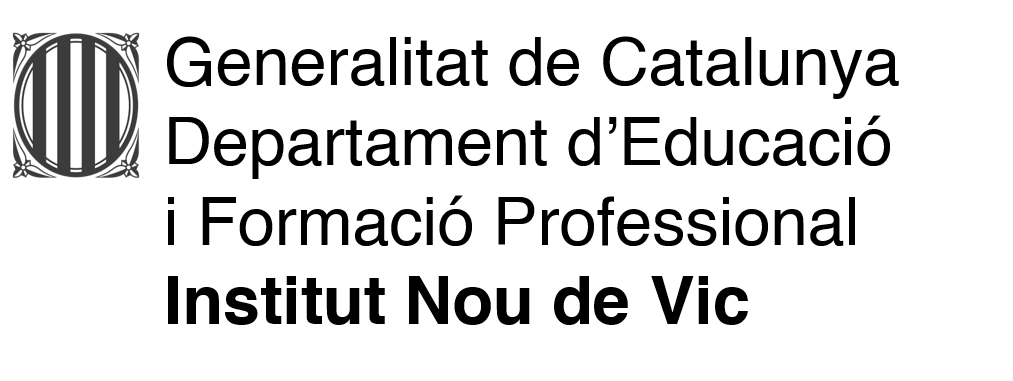
\includegraphics[height=1.8cm]{Logo_Departament.png}}
\fancyhead[R]{
\includegraphics[height=1.8cm]{Logo_Institut.png}}
\fancyfoot[C]{Pàgina \thepage\ de \pageref{LastPage}}
\renewcommand{\headrulewidth}{0.4pt}

\begin{document}

% --- CAPÇALERA D'IDENTIFICACIÓ ---
\begingroup
\renewcommand{\arraystretch}{2.2}
\begin{tabularx}{\textwidth}{|X|p{4cm}|}
    \hline
    \textbf{Nom i cognoms:} & \textbf{Grup:} \\ \hline
    \textbf{Activitat:} ACT-R1 & \textbf{Data: 2 de març 2025} \\ \hline
\end{tabularx}
\endgroup

\vspace{0.5cm}

\begin{center}
    {\Large \textbf{EXERCICIS MATEMÀTIQUES 1r BAT.}}\\[0.3em]
    {\normalsize La correcta resolució d'aquests exercicis i el seu puntual lliurament us pot apujar la nota fins a un màxim de \textbf{+0{,}5 punts}.}
\end{center}

\vspace{0.3cm}

% ============================================================
%  EXERCICI 1
% ============================================================
\begin{enumerate}[label=\textbf{\arabic*.}, leftmargin=*, itemsep=1.2em]

\item Donats el vector $\vec{v} = (7,-5)$ i els punts $A(-2,3)$ i $B(4,5)$, trobar:

\begin{enumerate}[label=\textbf{\alph*.}, itemsep=0.8em]

  \item Les equacions \textbf{contínua} i \textbf{general} de la recta que passa pels punts $A$ i $B$.

  \solucio{%
    El vector director $\overrightarrow{AB}$ és:
    \[
      \overrightarrow{AB} = B - A = (4-(-2),\; 5-3) = (6,\,2)
    \]
    \textbf{Equació contínua:}
    \[
      \frac{x-(-2)}{6} = \frac{y-3}{2}
      \quad\Longrightarrow\quad
      \boxed{\frac{x+2}{6} = \frac{y-3}{2}}
    \]
    \textbf{Equació general} (producte creuat i simplificació per 2):
    \[
      2(x+2) = 6(y-3)
      \;\Rightarrow\; 2x+4 = 6y-18
      \;\Rightarrow\;
      \boxed{x - 3y + 11 = 0}
    \]
  }

  \item Les equacions \textbf{paramètriques} i \textbf{explícita} de la recta que passa pel punt $A$
        i té com a vector director $\vec{v} = (7,-5)$.

  \solucio{%
    \textbf{Equacions paramètriques} (punt $A(-2,3)$, director $(7,-5)$):
    \[
      \boxed{\begin{cases} x = -2 + 7t \\ y = \phantom{-}3 - 5t \end{cases} \quad t\in\mathbb{R}}
    \]
    \textbf{Equació explícita}: aïllem $t$ de la primera equació:
    $t = \dfrac{x+2}{7}$, substituïm a la segona:
    \[
      y = 3 - 5\cdot\frac{x+2}{7} = \frac{21 - 5x - 10}{7}
      \quad\Longrightarrow\quad
      \boxed{y = -\tfrac{5}{7}\,x + \tfrac{11}{7}}
    \]
  }

  \item Les equacions \textbf{punt-pendent} i \textbf{canònica} de la recta que passa per $B$
        i té pendent $m = \dfrac{4}{3}$.

  \solucio{%
    \textbf{Equació punt-pendent} (punt $B(4,5)$, pendent $\frac{4}{3}$):
    \[
      \boxed{y - 5 = \frac{4}{3}(x-4)}
    \]
    El vector director associat al pendent $m = 4/3$ és $(3,4)$. L'\textbf{equació canònica}:
    \[
      \boxed{\frac{x}{\frac{1}{4}}-\frac{y}{\frac{1}{3}}=1}
    \]
  }

\end{enumerate}

% ============================================================
%  EXERCICI 2
% ============================================================
\item Per a cada apartat, determina la \textbf{posició relativa} del parell de rectes $r$ i $s$.
      En el cas que siguin secants, troba el punt on es tallen.

\begin{enumerate}[label=\textbf{\alph*.}, itemsep=0.8em]

  \item $r:\; -3x - 2y + 2 = 0$ \hfill
        $s:\; \dfrac{x-5}{4} = \dfrac{y-1}{-6}$

  \solucio{%
    Convertim $s$ a forma general: producte creuat:
    \[
      -6(x-5) = 4(y-1)
      \;\Rightarrow\; -6x+30 = 4y-4
      \;\Rightarrow\; 3x + 2y - 17 = 0
    \]
    Comparem les equacions generals:
    \[
      r:\; 3x + 2y - 2 = 0 \qquad s:\; 3x + 2y - 17 = 0
    \]
    Els coeficients de $x$ i $y$ són proporcionals ($\frac{3}{3}=\frac{2}{2}=1$)
    però els termes independents difereixen ($-2 \neq -17$).\\
    \textbf{Conclusió: les rectes són \underline{paral·leles} (no coincidents).}
  }

  \item $r:\; 4x - 7y + 3 = 0$ \hfill
        $s:\; y = -\dfrac{4}{5}\,x + 5$

  \solucio{%
    Convertim $s$ a forma general:
    \[
      5y = -4x + 25 \;\Rightarrow\; 4x + 5y - 25 = 0
    \]
    Comparem: $r$ té coeficients $(4, -7)$ i $s$ té $(4, 5)$.
    Com que $\frac{4}{4} \neq \frac{-7}{5}$, les rectes \textbf{no} són paral·leles.\\[4pt]
    \textbf{Conclusió: les rectes són \underline{secants}.} Resolem el sistema:
    \[
      \begin{cases} 4x - 7y + 3 = 0 \\ 4x + 5y - 25 = 0 \end{cases}
    \]
    Restem la primera de la segona:
    \[
      12y - 28 = 0 \;\Rightarrow\; y = \frac{28}{12} = \frac{7}{3}
    \]
    Substituïm a la primera: $4x = 7\cdot\frac{7}{3} - 3 = \frac{49-9}{3} = \frac{40}{3}
    \;\Rightarrow\; x = \frac{10}{3}$.\\[4pt]
    \textbf{Punt de tall:}
    $\displaystyle\boxed{\left(\frac{10}{3},\,\frac{7}{3}\right)}$
  }

\end{enumerate}

% ============================================================
%  EXERCICI 3
% ============================================================
\item Resoldre els següents \textbf{triangles}:

\begin{enumerate}[label=\textbf{\alph*.}, itemsep=0.8em]

  \item El triangle de costats $a = 150\text{ cm}$, $b = 166\text{ cm}$ i $c = 88\text{ cm}$.

  \solucio{%
    Tres costats coneguts $\Rightarrow$ apliquem el \textbf{teorema del cosinus} per trobar els angles.\\[4pt]
    \textbf{Angle $A$:}
    \[
      \cos A = \frac{b^2+c^2-a^2}{2bc}
             = \frac{166^2+88^2-150^2}{2\cdot166\cdot88}
             = \frac{27556+7744-22500}{29216}
             = \frac{12800}{29216} \approx 0{,}4381
    \]
    \[
      A = \arccos(0{,}4381) \approx \boxed{64{,}0°}
    \]
    \textbf{Angle $B$:}
    \[
      \cos B = \frac{a^2+c^2-b^2}{2ac}
             = \frac{150^2+88^2-166^2}{2\cdot150\cdot88}
             = \frac{22500+7744-27556}{26400}
             = \frac{2688}{26400} \approx 0{,}1018
    \]
    \[
      B = \arccos(0{,}1018) \approx \boxed{84{,}2°}
    \]
    \textbf{Angle $C$:}
    \[
      C = 180° - A - B \approx 180° - 64{,}0° - 84{,}2° \approx \boxed{31{,}8°}
    \]
    \textit{Comprovació: $64{,}0°+84{,}2°+31{,}8° = 180°$ ✓}
  }

  \item El triangle de costats $a = 12\text{ cm}$, $c = 19\text{ cm}$ i angle $\hat{B} = 30°$.

  \solucio{%
    Dos costats i l'angle comprès $\Rightarrow$ \textbf{teorema del cosinus} per al costat $b$:
    \[
      b^2 = a^2 + c^2 - 2ac\cos B
           = 144 + 361 - 2\cdot12\cdot19\cdot\cos 30°
           = 505 - 456\cdot\frac{\sqrt{3}}{2}
           \approx 505 - 394{,}77 \approx 110{,}23
    \]
    \[
      b \approx \boxed{10{,}50\text{ cm}}
    \]
    Ara apliquem el \textbf{teorema del sinus} per trobar $A$:
    \[
      \frac{\sin A}{a} = \frac{\sin B}{b}
      \;\Rightarrow\;
      \sin A = \frac{12\cdot\sin 30°}{10{,}50} = \frac{12\cdot 0{,}5}{10{,}50} \approx 0{,}5714
    \]
    \[
      A \approx \arcsin(0{,}5714) \approx \boxed{34{,}8°}
    \]
    (La solució obtusa $A'\approx145{,}2°$ no és vàlida ja que $B+A'>180°$.)
    \[
      C = 180° - 30° - 34{,}8° \approx \boxed{115{,}2°}
    \]
  }

\end{enumerate}

% ============================================================
%  EXERCICI 4
% ============================================================
\item Resoldre les equacions \textbf{trigonomètriques}:

\begin{enumerate}[label=\textbf{\alph*.}, itemsep=0.8em]
\item $\sin(3x) - 1 = 0$

\solucio{%
  \[
    \sin(3x) = 1
    \;\Rightarrow\;
    3x = 90° + 360°k,\quad k\in\mathbb{Z}
  \]
  \[
    \boxed{x = 30° + 120°k, \quad k\in\mathbb{Z}}
  \]
  \textit{Primeres solucions ($k=0,1,2$):
  $x = 30°,\; 150°,\; 270°,\;\ldots$}
}

\item $\tan^2 x + 2 = 5$

\solucio{%
  \[
    \tan^2 x = 3
    \;\Rightarrow\;
    \tan x = \pm\sqrt{3}
  \]
  \[
    \tan x = \sqrt{3} \;\Rightarrow\; x = 60° + 180°k
    \qquad
    \tan x = -\sqrt{3} \;\Rightarrow\; x = -60° + 180°k
    \quad k\in\mathbb{Z}
  \]
  \[
    \boxed{x = \pm 60° + 180°k,\quad k\in\mathbb{Z}}
  \]
  \textit{Primeres solucions: $x = 60°,\;120°,\;240°,\;300°,\;\ldots$}
}

\end{enumerate}

% ============================================================
%  EXERCICI 5
% ============================================================
\item Calcula a partir de les raons dels \textbf{angles notables}:

\begin{enumerate}[label=\textbf{\alph*.}, itemsep=0.8em]

  \item $\sin(135°)$

  \solucio{%
    $135° = 180° - 45°$ (segon quadrant, sinus positiu):
    \[
      \sin(135°) = \sin(180°-45°) = \sin(45°) = \boxed{\dfrac{\sqrt{2}}{2}}
    \]
  }

  \item $\cos(225°)$

  \solucio{%
    $225° = 180° + 45°$ (tercer quadrant, cosinus negatiu):
    \[
      \cos(225°) = \cos(180°+45°) = -\cos(45°) = \boxed{-\dfrac{\sqrt{2}}{2}}
    \]
  }

  \item $\tan(15°)$

  \solucio{%
    $15° = 45° - 30°$. Apliquem la fórmula de la diferència:
    \[
      \tan(45°-30°) = \frac{\tan 45° - \tan 30°}{1 + \tan 45°\cdot\tan 30°}
      = \frac{1 - \frac{1}{\sqrt{3}}}{1 + \frac{1}{\sqrt{3}}}
      = \frac{\sqrt{3}-1}{\sqrt{3}+1}
    \]
    Racionalitzem multiplicant per $(\sqrt{3}-1)$:
    \[
      = \frac{(\sqrt{3}-1)^2}{(\sqrt{3}+1)(\sqrt{3}-1)}
      = \frac{3 - 2\sqrt{3} + 1}{3 - 1}
      = \frac{4-2\sqrt{3}}{2}
      = \boxed{2 - \sqrt{3}}
    \]
  }

  \item $\cos(105°)$

  \solucio{%
    $105° = 60° + 45°$. Apliquem la fórmula de la suma:
    \[
      \cos(60°+45°) = \cos 60°\cos 45° - \sin 60°\sin 45°
      = \frac{1}{2}\cdot\frac{\sqrt{2}}{2} - \frac{\sqrt{3}}{2}\cdot\frac{\sqrt{2}}{2}
      = \frac{\sqrt{2}}{4} - \frac{\sqrt{6}}{4}
      = \boxed{\dfrac{\sqrt{2}-\sqrt{6}}{4}}
    \]
  }

\end{enumerate}

\end{enumerate}

\end{document}